\chapter{Time-Independent Schrodinger Equation}

\section{Exercises}

\exercise{2.1MOD}{
	Prove the following:
	\begin{itemize}
		\item For normalizable solutions, the separation constant E must be real. Hint: take $E = E_0+i\Gamma$, for real constants $\Gamma, E_0$.
		\begin{flalign*}
			\int_{\mathbb{R}}|\Psi|^2~dx&=1\\\\
			\Psi(x,t) &= \psi(x)e^{-\frac{i(E_0+i\Gamma)}{\hbar}t}\\
			|\Psi(x,t)|^2 &= \Psi^*\Psi = \psi^*e^{\frac{iE_0}{\hbar}t}e^{\frac{\Gamma}{\hbar}t}\psi e^{\frac{-iE_0}{\hbar}t}e^{\frac{\Gamma}{\hbar}t}\\
			&= \psi^*\psi e^{\frac{2\Gamma}{\hbar}t} = |\psi(x)|^2 e^{\frac{2\Gamma}{\hbar}t}\\
			\int_{\mathbb{R}}|\Psi|^2~dx &= e^{\frac{2\Gamma}{\hbar}t} \int_{\mathbb{R}}|\psi(x)|^2~dx = 1~\forall t\impliedby e^{\frac{2\Gamma}{\hbar}t} = C \implies \Gamma = 0
		\end{flalign*}
		\item The time-independent wave function $\psi(x)$ can always be taken to be real (unlike $\Psi(x,t)$). This doesn't mean that every solution to the time-ind. Schro equation is real; what it says 
		is that if you've got one that is not, it can always be expressed as a linear combination of solutions (with the same energy) that are. So you might as well stick to $\psi$s that are real.
		\begin{flalign*}
			f(x) &= a+ib, ~a,b \in \mathbb{R}\\
			f(x)+f^*(x) &= 2a \implies a = \frac{f(x)+f^*(x)}{2}\\
			f(x)-f^*(x) &= 2ib\implies b = -i\frac{f(x)-f^*(x)}{2}\\
			-\frac{\hbar^2}{2m}\derivative[2]{\psi}{x}+(V(x)-E)\psi(x) &= 0 = -\frac{\hbar^2}{2m}\derivative[2]{\psi^*}{x}+(V(x)-E)\psi^*(x)\\
		\end{flalign*}
		This last line shows the form for linear, homogeneous ODEs for which their weighted sum also serves as a solution to the original ODE. To get the values for the constants $c$, then we can use $c_1 = c_2 = 1/2$ values for real solutions implied by $a$, or $c_1 = -i/2,~c_2 = i/2$ for real solutions implied by $b$ as well:
		\begin{flalign*}
			f(x) = \psi(x)=c_1\psi(x)+c_2\psi^*(x)
		\end{flalign*}
		If $\psi(x)$ did not have any imaginary term(s), then one would pick any real constants to produce a real solution. Hence, if the solutions for the complex conjugate and the conjugate satisfy the time-ind. Schro for real $E, V(x)$, any linear combination of these will also follow suit. 
		Note that $$\psi = \frac{1}{2}((\psi+\psi^*)+i(-i(\psi-\psi^*)))$$ which shows $\psi$ can be written as a linear combination of two real solutions $\psi+\psi^*$ and $i(\psi-\psi^*)$.  Recall that the complex number system extends the real numbers with the imaginary unit $i$ satisfying $i^2=-1$.
		\item If $V(x)$ is an even function (i.e., $V(-x)=V(x)$), then $\psi(x)$ can always be taken to be either even or odd.
		\begin{flalign*}
			x = -y &\implies -\derivative{y}{x}=1\\
			\derivative{\psi(x)}{x} &= \derivative{\psi(-y)}{(-y)}\cancelto{1}{\derivative{(-y)}{x}}= -\derivative{\psi(-y)}{y}\\
			\derivative[2]{\psi(x)}{x} &= \derivative{}{x}\derivative{\psi}{x} = -\cancelto{1}{\derivative{(-y)}{x}}\derivative{}{(-y)}\derivative{\psi(-y)}{y} = \derivative[2]{\psi(-y)}{y}
		\end{flalign*}
		Now substitute as needed,
		\begin{flalign*}
			-\frac{\hbar^2}{2m}\derivative[2]{\psi(-y)}{(-y)}+(V(-y)-E)\psi(-y) &= -\frac{\hbar^2}{2m}\derivative[2]{\psi(x)}{x}+(V(x)-E)\psi(x)  = 0\\
		\end{flalign*}
		As before, we get a linear ODE for the even-odd pair whose weighted sum also produces a real solution as discussed prior $$\psi(x)=c_1\psi(-x)+c_2\psi(x)$$ Thus, any (real) solution can be expressed as a linear combination of even or odd solutions given an even potential well function with $c_1 = c_2 = 1$ producing a possible even function or $c_1=-1,~c_2=1$ producing a possible odd function, $$f_e=\frac{f(x)+f(-x)}{2},~f_o=\frac{f(x)-f(-x)}{2}$$
		 It's important to note that when dealing with a real physical system, the wave function is generally a complex-valued function. However, the even and odd classifications refer
		 to the symmetry properties of the real part of the wave function. We add the ``wiggle factor'' when including time domain considerations that gets us into imaginary land.\\
		\item Does the prior statement hold for an odd potential function?\\\\
		Here, the probability density of finding the particle is opposite on both sides of the origin. This occurs when the particle's state possesses spatial asymmetry. The statement does not hold for an odd potential well function, where we would strictly need an odd wave function $\psi(x)=-\psi(-x)$ to maintain the proper relation above; an even wave function would contradict the antisymmetric nature of the potential function in this case.  
	\end{itemize}
}

\exercise{2.2}{
	Show that $E$ must exceed the minimum value of $V(x)$, for every normalizable solution to the time-ind Schro. What is the classical analog to this statement?
	
	\begin{equation*}
	-\frac{\hbar^2}{2m}\derivative[2]{\psi}{x}+V(x)\psi=E\psi
	\end{equation*}
			
	Assume that there exists a normalizable solution $\psi(x)$ to the time-independent Schrödinger equation with energy $E$ that satisfies $E < V(x)_{min}$, where $V(x)_{min}$ is the minimum value of the potential energy function $V(x)$. Then we can write:
	
	\begin{equation*}
		E\psi = -\frac{\hbar^2}{2m}\derivative[2]{\psi}{x}+V(x)\psi < V(x)_{min}\psi
	\end{equation*}
	
	Dividing both sides by $\psi$ and rearranging, we get:
	
	\begin{equation*}
	-\frac{\hbar^2}{2m}\derivative[2]{\psi}{x}+(V(x)-V(x)_{min})\psi < 0
	\end{equation*}
	
	Since $\psi$ is normalizable, it must approach zero as $x$ approaches infinity or negative infinity; if we knew the function of $V(x)$ and set $D = V(x)-V(x)_{min}$ and solved for $\psi(x)$, we would get an expression in terms of $x$:
	 

	\begin{flalign*}
		-\frac{\hbar^2}{2m}\derivative[2]{\psi}{x}+D\psi &= k,~k \in \mathbb{R}~(in~Joules,~\psi~dimensionless!)\\
		\psi(x) &= \begin{cases}
			c_1e^{-\frac{\sqrt{2Dm}}{\hbar}x}+c_2e^{\frac{\sqrt{2Dm}}{\hbar}x} & \text{if } k = 0 \impliedby \psi = 0,~E \nless 0 \text{ (see: ZPT, and exception QNEC)} \\
			c_3e^{-\frac{\sqrt{2Dm}}{\hbar}x}+c_4e^{\frac{\sqrt{2Dm}}{\hbar}x}-\frac{|k|}{D} & \text{if } k < 0\\
		\end{cases}
	\end{flalign*}
	 
	 
	Both cases allow us to find constants for the normalization condition to hold. When $x \rightarrow \infty$ then $\psi(x) \rightarrow \infty$. When $x \rightarrow -\infty$ then $\psi(x) \rightarrow -\infty$.
	This implies that any further derivatives have the same sign in these regions. By indicating the negation, we are counteracting the growth of $\psi$ to ``head back'' towards 0, therefore, the negated second derivative term must be zero
	 (when we have non-normalizable $\psi$ = 0, where the probability of finding the system in any particular state is not well-defined) or negative (substituting in $\pm \infty$ always yields a positive second derivative and we need a real solution -- $D>0$ as we shall soon see) for all values of $x$,
	
	\begin{equation*}
	-\frac{\hbar^2}{2m}\derivative[2]{\psi}{x} \leq 0
	\end{equation*}
	
	Combining this with the previous inequality, we get:
	
	\begin{equation*}
	D = (V(x)-V(x)_{min}) < 0
	\end{equation*}
	
	But this contradicts the fact that $V(x)_{min}$ is the minimum value of $V(x)$, which means that $V(x)-V(x)_{min}$ is non-negative for all values of $x$. Also note this would otherwise produce
	 complex-valued solutions to $\psi(x)$. Therefore, our initial assumption that $E < V(x)_{min}$ must be false, and we can conclude that $E$ must meet or exceed the minimum value of $V(x)$ for every normalizable solution to the time-independent Schrödinger equation.

	If the energy is equal to or less than the potential energy at a certain point, the particle would be confined to that region (held by an ``infinite force'') 
	and unable to escape. This situation would violate the classical principle of conservation of energy, which states that the total energy of a system is conserved
	 and cannot be created or destroyed. In this case, the particle would have less energy than the potential energy barrier, and therefore, energy conservation would be
	violated. A more sophisticated analysis can be done by showing this violates the principle of least action: the particle would be in a region where its kinetic energy
	is negative or zero, leading to an imaginary or zero action. However, the principle of least action requires that the action be minimized, which corresponds to a
	 real, non-zero value (proof beyond scope of intro course).\\\\
}

\exercise{2.3}{
	Show that there is no acceptable solution to the (time-ind.) Schro for the infinite square well with $E = 0$ or $E < 0$.
	\begin{flalign*}
		\text{Case where } E &= 0:\\
		\pdv[2]{\psi}{x}&=-\frac{2mE}{\hbar^2}\psi = 0 \implies \psi(x) = Ax+B\\
		\psi(0)&=\psi(a)=0 \implies B = 0 \implies \psi(x) = Ax = 0
	\end{flalign*}
	We get a non-normalizable result $\psi(x) = 0$ whereby any constant of integration becomes a normalization factor, whose simultaneity is nonsensical.
	\begin{flalign*}
		\text{Case where } E < 0:\\
		\pdv[2]{\psi}{x}&=\frac{2mE}{\hbar^2}\psi \implies \psi(x) = Ae^{-\frac{\sqrt{2mE}}{\hbar}x}+Be^{\frac{\sqrt{2mE}}{\hbar}x}\\
		\psi(0)&=0 \implies B = 0 \implies A = -B\\
		\psi(a)&=0,~A=-B \implies B = 0 ~|~\frac{\sqrt{2mE}}{\hbar}x = -\frac{\sqrt{2mE}}{\hbar}x \implies \frac{\sqrt{2mE}}{\hbar} = 0\\
	\end{flalign*}
	In this case all roads lead to having $\psi(x) = 0$ again, which is a non-normalizable solution.
}\\

\exercise{2.4}{
	Calculate $\langle x \rangle,~\langle x^2 \rangle,~\langle p \rangle,~\langle p^2 \rangle,~\sigma_x,~\sigma_p$ for the $n^{th}$ stationary state for the infinite square well. Check that the uncertainty principle is satisfied. Which state comes closest to the uncertainty limit?
	\begin{flalign*}
		\langle x \rangle = \int x|\psi^2|~dx= \frac{2}{a}\int_0^a x\sin^2\bigl(\frac{n\pi x}{a}\bigr)~dx &= \frac{1}{a}\int_0^a x\bigl(1-\cos\bigl(\frac{2n\pi x}{a}\bigr))~dx\\
		&= \frac{1}{a}\int_0^a x-x\cos\bigl(\frac{2n\pi x}{a}\bigr)~dx\\
		&= \frac{a}{2}-\frac{1}{a}\int_0^a x\cos\bigl(\frac{2n\pi x}{a}\bigr)~dx \\
		& = \frac{a}{2}+\cancelto{0}{\frac{x\sin\bigl(\frac{2n\pi x}{a}\bigr)}{2 \pi n}\Biggr|_0^a}-\frac{1}{2 \pi n}\int_0^a \sin \bigl(\frac{2 \pi n x}{a}\bigr)~dx\\
		&= \frac{a}{2} + \frac{a}{4 \pi^2 n^2}\int_0^{2\pi n}\sin(u)~du = \frac{a}{2} + \cancelto{0}{\frac{a}{4 \pi^2 n^2}\cos(u)\Biggr|_0^{2 \pi n}}\\
		&= \frac{a}{2}\\
		\langle x^2 \rangle = \int x^2|\psi^2|~dx= \frac{2}{a}\int_0^a x^2\sin^2\bigl(\frac{n\pi x}{a}\bigr)~dx &= \frac{1}{a}\int_0^a x^2\bigl(1-\cos\bigl(\frac{2n\pi x}{a}\bigr))~dx\\
		&= \frac{1}{a}\int_0^a x^2-x^2\cos\bigl(\frac{2n\pi x}{a}\bigr)~dx\\
		&=\frac{1}{a}\Biggl[\frac{x^3}{3}\Biggr|_0^a - \int_0^a x^2\cos \frac{2 n \pi x}{a}~dx\Biggr] = \frac{1}{a}\Biggl[\frac{a^3}{3} - \frac{a^3}{8n^3\pi^3}\int_0^{2 n \pi} y^2\cos y~dy\Biggr]\\
		&= \frac{1}{a}\Biggl[\frac{a^3}{3} - \frac{a^3}{8n^3\pi^3}\Biggl(\cancelto{0}{y^2\sin y \Biggr|_0^{2 n \pi}} - 2\int_0^{2n\pi}y \sin y ~dy\Biggr)\Biggr]\\
		&= \frac{1}{a}\Biggl[\frac{a^3}{3} - \frac{a^3}{8n^3\pi^3}\Biggl(2y\cos y \Biggr|_0^{2 n \pi}-\cancelto{0}{2 \sin y  \Biggr|_0^{2 n \pi}}\Biggr)\Biggr]\\
		&= \frac{a^2}{3}-\frac{a^2}{2n^2\pi^2} = a^2\Biggl(\frac{1}{3}-\frac{1}{2n^2\pi^2}\Biggr)\\
		\sigma_x = \sqrt{\langle x^2 \rangle - \langle x \rangle^2} &= \frac{a}{2}\sqrt{\frac{1}{3}-\frac{2}{n^2\pi^2}}\\
		\langle p \rangle &= -i\hbar \int_0^a \psi_n^*\pdv{\psi_n}{x}~dx = m\derivative{\langle x \rangle}{t} = 0\\
		\langle p^2 \rangle &= \int_0^a \psi_n^*\Biggl[-i\hbar\derivative{}{x}\Biggr]^2\psi_n~dx = -\hbar^2 \int_0^a \psi_n^* \derivative[2]{\psi_n}{x}~dx\\
		&= \hbar^2 \int_0^a \psi_n^* k^2\psi_n~dx ~~(by~2.24)\\
		&= \frac{2mE_n\hbar^2}{\hbar^2}\int_0^a \psi_n^*\psi_n~dx = 2mE_n = \Biggl(\frac{n \pi \hbar}{a}\Biggr)^2~~(\psi s~orthonormal)\\
		\sigma_p &= \sqrt{\langle p^2 \rangle - \langle p \rangle^2} =\frac{n \pi \hbar}{a}\\
		\sigma_p\sigma_x &= \frac{\hbar}{2}\sqrt{\frac{n^2\pi^2}{3}-2} \geq \frac{\hbar}{2}\\
	\end{flalign*}
	Note that the complex-valued time dependence was ``dropped'' as those terms cancel out. The product is smallest for state $n=1$, $1.136\hbar/2$.
}
\exercise{2.5}{
	A particle in the infinite square well has its initital wave function an even mixture of the first two stationary states: $$\Psi(x,0)=A\Biggl[\psi_1(x)+\psi_2(x)\Biggr]$$ 
	\begin{itemize}
		\item Normalize $\Psi(x,0)$. Recall that, having normalized $\Psi$ at $t = 0$, you can rest assured that it stays normalized -- you can check this explicity after the next item.
			\begin{flalign*}
				1 &= \int \Psi\Psi^*~dx = |A|^2 \int (\psi_1^*+\psi_2^*)(\psi_1+\psi_2)~dx = |A|^2 \int |\psi_1|^2+|\psi_2|^2 +\psi_1^*\psi_2+\psi_2^*\psi_1~dx\\
				&= |A|^2(1+1+0+0)~~(orthonormality)\\
				A &= \frac{1}{\sqrt{2}}\\
				\Psi(x,0)&=\underbrace{\frac{1}{\sqrt{2}}}_{c_n}\Biggl[\psi_1(x)+\psi_2(x)\Biggr]
			\end{flalign*}
		\item Find $\Psi(x,t)$, $|\Psi(x,t)|^2$. Express the latter as a sinusoidal function of time. To simplify, let $\omega = \frac{\pi^2 \hbar}{2ma^2}$.
			\begin{flalign*}
				\Psi(x,t) &= \sum_{n=1}^2 c_n\psi_n e^{-\frac{iE_n}{\hbar}t} = \sum_{n=1}^2 c_n\Psi(x,t) \impliedby \hbar n^2 \omega = E_n\\
				\Psi(x,t) &= \frac{1}{\sqrt{2}}\Biggl[\psi_1(x)e^{-\frac{i \hbar \pi^2}{2ma^2}t}+\psi_2(x)e^{-\frac{4i \hbar \pi^2}{2ma^2}t}\Biggr] = \frac{1}{\sqrt{2}}\Biggl[\psi_1(x)e^{-i \hbar \omega t}+\psi_2(x)e^{-4i \omega t}\Biggr]\\
				&= \frac{1}{\sqrt{2}}\sqrt{\frac{2}{a}}\Biggl(\sin\frac{\pi x}{a} e^{-i\omega t}+\sin \frac{2 \pi x}{a}e^{-4i \omega t}\Biggr) = \frac{e^{-i \omega t}}{\sqrt{a}}\Biggl(\sin \frac{\pi x}{a}+\sin \frac{2 \pi x}{a}e^{-3i \omega t}\Biggr)\\
				|\Psi(x,t)|^2 &= \frac{1}{a}\Biggl(\sin^2 \frac{\pi x}{a}+\sin \frac{2 \pi x}{a}\sin \frac{\pi x}{a}(e^{-3i \omega t}+e^{3 i \omega t})+\sin^2 \frac{2 \pi x}{a}\Biggr)\\
				&= \frac{1}{a}\Biggl(\sin^2 \frac{\pi x}{a} + \sin^2 \frac{2 \pi x }{a} + 2 \sin \frac{\pi x}{a}\sin \frac{2 \pi x}{a}\cos 3\omega t\Biggr)
			\end{flalign*}
		\item Compute $\langle x \rangle$. Notice it oscillates in time. What is the angular frequency of this oscillation? What is the amplitude of oscillation? (If your amplitude is greater than $a/2$, go directly to jail)
			\begin{flalign*}
				\langle x \rangle &= \int x |\Psi|^2 ~dx = \frac{1}{a} \int_0^a x\Biggl(\sin^2 \frac{\pi x}{a} + \sin^2 \frac{2 \pi x }{a} + 2 \sin \frac{\pi x}{a}\sin \frac{2 \pi x}{a}\cos 3\omega t\Biggr)~dx\\
				&= \frac{a}{2}\Biggl(1-\frac{32}{9\pi^2}\cos(3 \omega t)\Biggr)~~(use~trig.~~sum~identities~and~IBP)\\
				Amplitude&:~\frac{a}{2}\frac{32}{9\pi^2}\\
				Angular~Frequency&:~3\omega = 3\frac{E_n}{\hbar n^2} = 3\frac{\pi^2 \hbar}{2 m a^2}
			\end{flalign*}
		\item Compute $\langle p \rangle$.
			\begin{flalign*}
				\langle p \rangle &= m\derivative{\langle x \rangle}{t} = \frac{8 \hbar}{3a}\sin(3 \omega t)
			\end{flalign*}
		\item If you measured the energy of this particle, what values might you get, and what is the probability of getting each of them? Find $\langle H \rangle$. How does it compare with $E_1$ and $E_2$?
			\begin{flalign*}
				\langle H \rangle &= \sum_{n=1}^2 |c_n|^2 E_n = |c_1|^2E_1+|c_2|^2E_2=P_1E_1+P_2E_2 = |1/\sqrt{2}|^2\frac{\pi^2\hbar^2}{2ma^2}+|1/\sqrt{2}|^2\frac{4\pi^2\hbar^2}{2ma^2}  = \frac{1}{2}(E_1+E_2) = \frac{5\pi^2\hbar^2}{4ma^2} 
			\end{flalign*}
			We see that the expectation value of the definite total energy (Hamiltonian) is the average of both excited states in this case.
	\end{itemize}
}

\exercise{2.6}{
	Although the overall phase constant of the wave function is of no physical significance (it cancels out whenever you calculate a measurable quantity), the relative phase of the coefficients of Eqn. 2.17 does matter. For example, suppose we change the relative phase from before:
	$$\Psi(x,0)=A\Biggl[\psi_1(x)+e^{i\phi}\psi_2(x)\Biggr],$$ where $\phi$ is some constant. Find $\Psi(x,t)$, $|\Psi(x,t)|^2$, and $\langle x \rangle$. Study the special case $\phi = \pi/2$ and $\phi = \pi$. Compare with results prior.
	\begin{flalign*}
		A &= \frac{1}{\sqrt{2}}\\
		\Psi(x,t) &= \frac{e^{-i \omega t}}{\sqrt{a}}\Biggl[\sin \frac{\pi x}{a} + \sin \frac{2\pi x }{a} e^{i(\phi-3\omega t)}\Biggr]\\
		|\Psi(x,t)|^2 &= \frac{1}{a}\Biggl[\sin^2 \frac{\pi x}{a} + \sin^2 \frac{2\pi x }{a} + 2 \sin \frac{2\pi x }{a} \sin \frac{\pi x }{a}\cos (3\omega t - \phi)\Biggr]\\
		\langle x \rangle &= \frac{a}{2}\Biggl[1-\frac{32}{9 \pi^2}\cos(3 \omega t - \phi)\Biggr]\\
		\phi = \frac{\pi}{2} &\implies \Psi(x,0) = \frac{1}{\sqrt{2}}\bigl[\psi_1(x)+i\psi_2(x)\bigr]\\
		& \implies \langle x \rangle = \frac{a}{2}\Biggl[1-\frac{32}{9 \pi^2}\sin(3 \omega t)\Biggr]\\
		&\implies \langle x \rangle = \frac{a}{2},~t = 0~(start~time)\\
		\phi = \pi &\implies \Psi(x,0) = \frac{1}{\sqrt{2}}\bigl[\psi_1(x)-\psi_2(x)\bigr]\\
		& \implies \langle x \rangle = \frac{a}{2}\Biggl[1+\frac{32}{9 \pi^2}\cos(3 \omega t)\Biggr]\\
		&\implies \langle x \rangle = \frac{a}{2}\biggl[1+\frac{32}{9 \pi^2}\biggr],~t = 0~(start~time)\\
	\end{flalign*}
	The relative phase of the coefficients $\{c_n\}$ allow us to shift the starting point when measuring the expectation value of position.
}

\exercise{2.7MOD}{
	A particle in an infinite square well has the initial wave function 
	\begin{flalign*}
		\Psi(x,0) = \begin{cases}
			Ax, & 0 \leq x \leq a\\
			A(a-x), & a/2 \leq x \leq a
		\end{cases}
	\end{flalign*}
	\begin{itemize}
		\item Sketch this out and determine normalization constant.
			\begin{flalign*}
				1 &= \int |\Psi|^2~dx = \int \Psi^*\Psi ~dx = |A|^2\Biggl[\int_0^{a/2}x^2~dx + \int_{a/2}^a (a-x)^2~dx\Biggr] \implies A = \frac{2 \sqrt{3}}{\sqrt{a^3}}
			\end{flalign*}
			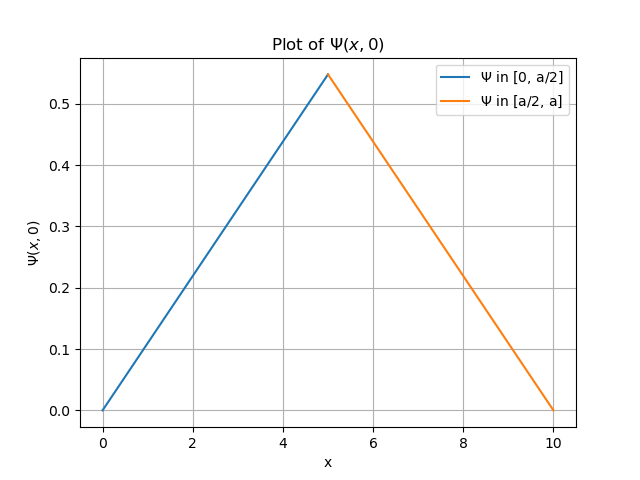
\includegraphics[width=\textwidth]{./chapters/graphs_ch2/2_7_1.png}
		\item Find $\Psi(x,t)$.
			\begin{flalign*}
				\Psi(x,t) =& \sum_{n=1}^\infty c_n\psi_n(x)e^{-\frac{iE_nt}{\hbar}} = \sum_{n=1}^\infty c_n \Psi_n(x,t)\\
				c_n &= \sqrt{\frac{2}{a}}\int_0^a \sin \frac{n \pi x}{a}\Psi(x,0)~dx = \frac{2 \sqrt{3}}{\sqrt{a^3}}\sqrt{\frac{2}{a}} \Biggl[\int_0^{a/2}x\sin \frac{\pi n x}{a}~dx + \int_{a/2}^{a}(a-x)\sin \frac{\pi n x}{a}~dx\Biggr]\\
				&= \frac{4 \sqrt{6}}{n^2\pi^2} \sin \frac{n \pi}{2} = \begin{cases}
					(-1)^{\frac{n-1}{2}}\frac{4 \sqrt{6}}{n^2\pi^2}, & n \text{ odd}\\
					0, & n \text{ even}
				\end{cases}\\
				\therefore \Psi(x,t) &= \frac{4 \sqrt{6}}{\pi^2} \sqrt{\frac{2}{a}} \sum_{1,3,5,\ldots} \frac{(-1)^{\frac{n-1}{2}}}{n^2}\sin \frac{n \pi x}{a}e^{-\frac{iE_nt}{\hbar}}\\
				E_n &= \frac{n^2\pi^2\hbar^2}{2ma^2}
			\end{flalign*}
		\item What is the probability that the measurement of the energy would yield a value $E_1$?
			\begin{flalign*}
				|c_1|^2 = 0.9855
			\end{flalign*}
		\item Find the expectation value of the energy, using Eqn. 2.21.
			\begin{equation*}
				\langle H \rangle = \sum_{n=1,3,5,\ldots}^\infty |c_n|^2E_n = \frac{96\hbar^2}{2ma^2 \pi^2}\Biggl(\frac{1}{1^2}+\frac{1}{3^2}+\frac{1}{5^2}+\ldots\Biggr) = \frac{96\hbar^2}{2ma^2 \pi^2}\underbrace{(1-2^{-2})\zeta(2)}_{\frac{\pi^2}{8}} = \frac{6 \hbar^2}{ma^2} 
			\end{equation*}
		\item Determine how the Fourier Transform, Riemann's Zeta Function, and Basel problem are related.
		\\\\Consider the Basel problem. We can express a function using the Fourier Transform. Consider the function $x^2$ that is continuos and differentiable on $[-L,L]=[-\pi, \pi]$.\\
		\begin{flalign*}
			f(x) &= \frac{a_0}{2}+\sum_{n=1}^{\infty}\Biggl(a_n\cos\frac{n \pi x }{L}+b_n\sin\frac{n \pi x }{L}\Biggr)\\
			\frac{a_0}{2} &= \frac{1}{2L}\int_{-L}^Lf(x)~dx = \frac{2}{2 \pi} \int_0^\pi x^2~dx = \frac{\pi^2}{3}\\
			a_n &= \frac{1}{L} \int_{-L}^{L} f(x) \cos \frac{n \pi x}{L}~dx = \frac{2}{\pi} \int_0^\pi x^2 \cos(n x) ~dx = \frac{4}{n^2}(-1)^n\\
			b_n &= \frac{1}{L} \int_{-L}^{L} f(x) \sin \frac{n \pi x}{L}~dx = \frac{1}{\pi} \int_{-\pi}^\pi x^2 \sin(n x) ~dx = 0\\
			f(\pi) = \pi^2 &= \frac{\pi^2}{3} + \sum_{n=1}^{\infty} \frac{4(-1)^n}{n^2}\cancelto{(-1)^n}{\cos(\pi n)} \iff 4 \sum_{n=1}^{\infty}\frac{1}{n^2}= \frac{2 \pi^2}{3} \implies \sum_{n=1}^{\infty}\frac{1}{n^2} = \frac{\pi^2}{6} \\
			f(0) = 0 &= \frac{\pi^2}{3} + \sum_{n=1}^{\infty} \frac{4(-1)^n}{n^2}\cancelto{1}{\cos(0)} \iff - \sum_{n=1}^{\infty}\frac{(-1)^n}{n^2} = \sum_{n=1}^{\infty}\frac{(-1)^{n+1}}{n^2} = \frac{\pi^2}{12}\\
		\end{flalign*}
		The last two last lines are two such ``problems'' and note how we can take different functions to determine coefficients which the below will also show. Euler did the above differently (see YouTube) but now we can turn to Riemann's Zeta Function.
		\begin{flalign*}
			\frac{\pi^2}{6} &= \frac{1}{1^2}+\frac{1}{2^2}+\frac{1}{3^2}+\ldots\\
			\frac{1}{2^2}\frac{\pi^2}{6} &= \frac{1}{2^2}+\frac{1}{4^2}+\frac{1}{6^2}+\ldots\\
			(1-\frac{1}{2^2})\frac{\pi^2}{6} &= \frac{1}{1^2}+\frac{1}{3^2}+\frac{1}{5^2}+\ldots =\frac{\pi^2}{8}\\
			(1-\frac{2}{2^2})\frac{\pi^2}{6} &= \frac{1}{1^2}-\frac{1}{2^2}+\frac{1}{3^2}-\frac{1}{4^2}+\ldots=\frac{\pi^2}{12}\\
		\end{flalign*}
		Now, generalize.
		\begin{flalign*}
			\zeta(z) = \frac{\pi^2}{6} &= \frac{1}{1^z}+\frac{1}{2^z}+\frac{1}{3^z}+\ldots\\
			(1-\frac{1}{2^z})\zeta(z) &= \frac{1}{1^z}+\frac{1}{3^z}+\frac{1}{5^z}+\ldots\\
			\frac{1}{2^z}\zeta(z) &= \frac{1}{2^z}+\frac{1}{4^z}+\frac{1}{6^z}+\ldots\\
			(1-\frac{2}{2^z})\frac{\pi^2}{6} &= \frac{1}{1^z}-\frac{1}{2^z}+\frac{1}{3^z}-\frac{1}{4^z}+\ldots\\
		\end{flalign*}
		Note for the harmonic series case, we may assume it converges. With this in mind, the second line below produces a greater sum, which we assume also converges. But, the sum of this line must be the sum of the last line, which is greater still. Thus, our initial assumption was wrong and all of them must diverge.
		\begin{flalign*}
			\zeta(1) &= \frac{1}{1}+\frac{1}{2}+\frac{1}{3}+\ldots = \infty\\
			(1-0.5)\zeta(1) &= \frac{1}{1}+\frac{1}{3}+\frac{1}{5}+\ldots = 0.5 \zeta(1) = \infty\\
			0.5 \zeta(1) &= \frac{1}{2}+\frac{1}{4} +\frac{1}{6}+\ldots = \infty\\
		\end{flalign*}
	\end{itemize}
}